%  LaTeX support: latex@mdpi.com 
%  In case you need support, please attach all files that are necessary for compiling as well as the log file, and specify the details of your LaTeX setup (which operating system and LaTeX version / tools you are using).

% You need to save the "mdpi.cls" and "mdpi.bst" files into the same folder as this template file.

%=================================================================
\documentclass[ijgi,article,submit,moreauthors,pdftex,10pt,a4paper]{Definitions/mdpi} 
\usepackage{subfig}

% If you would like to post an early version of this manuscript as a preprint, you may use preprint as the journal and change 'submit' to 'accept'. The document class line would be, e.g. \documentclass[preprints,article,accept,moreauthors,pdftex,10pt,a4paper]{mdpi}. This is especially recommended for submission to arXiv, where line numbers should be removed before posting. For preprints.org, the editorial staff will make this change immediately prior to posting.

%
%--------------------
% Class Options:
%--------------------
% journal
%----------
% Choose between the following MDPI journals:
% acoustics, actuators, addictions, admsci, aerospace, agriculture, agronomy, algorithms, animals, antibiotics, antibodies, antioxidants, applsci, arts, asi, atmosphere, atoms, axioms, batteries, bdcc, behavsci, beverages, bioengineering, biology, biomedicines, biomimetics, biomolecules, biosensors, brainsci, buildings, carbon, cancers, catalysts, cells, ceramics, challenges, chemengineering, chemosensors, children, cleantechnol, climate, clockssleep, cmd, coatings, colloids, computation, computers, condensedmatter, cosmetics, cryptography, crystals, cybersecurity, data, dentistry, designs, diagnostics, dairy, diseases, diversity, drones, econometrics, economies, education, electrochem, electrochemistry, electronics, energies, entropy, environments, epigenomes, est, fermentation, fibers, fire, fishes, fluids, foods, forecasting, forests, fractalfract, futureinternet, galaxies, games, gastrointestdisord, gels, genealogy, genes, geohazards, geosciences, geriatrics, hazardousmatters, healthcare, heritage, highthroughput, horticulturae, humanities, hydrology, informatics, information, infrastructures, inorganics, insects, instruments, ijerph, ijfs, ijms, ijgi, ijtpp, inventions, j, jcdd, jcm, jcs, jdb, jfb, jfmk, jimaging, jof, jintelligence, jlpea, jmmp, jmse, jpm, jrfm, jsan, land, languages, laws, life, literature, logistics, lubricants, machines, magnetochemistry, make, marinedrugs, materials, mathematics, mca, medsci, medicina, medicines, membranes, metabolites, metals, microarrays, micromachines, microorganisms, minerals, modelling, molbank, molecules, mps, mti, nanomaterials, ncrna, neonatalscreening, neuroglia, nitrogen, nutrients, ohbm, particles, pathogens, pharmaceuticals, pharmaceutics, pharmacy, philosophies, photonics, plants, plasma, polymers, polysaccharides, proceedings, processes, proteomes, publications, quaternary, qubs, reactions, recycling, religions, remotesensing, reports, resources, risks, robotics, safety, sci, scipharm, sensors, separations, sexes, sinusitis, smartcities, socsci, societies, soilsystems, sports, standards, stats, surfaces, surgeries, sustainability, symmetry, systems, technologies, toxics, toxins, tropicalmed, universe, urbansci, vaccines, vehicles, vetsci, vibration, viruses, vision, water, wem, wevj
%---------
% article
%---------
% The default type of manuscript is article, but can be replaced by: 
% abstract, addendum, article, benchmark, book, bookreview, briefreport, casereport, changes, comment, commentary, communication, conceptpaper, correction, conferenceproceedings, conferencereport, expressionofconcern, meetingreport, creative, datadescriptor, discussion, editorial, essay, erratum, hypothesis, interestingimages, letter, meetingreport, newbookreceived, opinion, obituary, projectreport, reply, reprint, retraction, review, perspective, protocol, shortnote, supfile, technicalnote, viewpoint
% supfile = supplementary materials
% protocol: If you are preparing a "Protocol" paper, please refer to http://www.mdpi.com/journal/mps/instructions for details on its expected structure and content.
%----------
% submit
%----------
% The class option "submit" will be changed to "accept" by the Editorial Office when the paper is accepted. This will only make changes to the frontpage (e.g. the logo of the journal will get visible), the headings, and the copyright information. Also, line numbering will be removed. Journal info and pagination for accepted papers will also be assigned by the Editorial Office.
%------------------
% moreauthors
%------------------
% If there is only one author the class option oneauthor should be used. Otherwise use the class option moreauthors.
%---------
% pdftex
%---------
% The option pdftex is for use with pdfLaTeX. If eps figures are used, remove the option pdftex and use LaTeX and dvi2pdf.

%=================================================================
\firstpage{1} 
\makeatletter 
\setcounter{page}{\@firstpage} 
\makeatother
\pubvolume{xx}
\issuenum{1}
\articlenumber{1}
\pubyear{2018}
\copyrightyear{2018}
\externaleditor{Academic Editor: name}
\history{Received: date; Accepted: date; Published: date}
%\updates{yes} % If there is an update available, un-comment this line

%------------------------------------------------------------------
% The following line should be uncommented if the LaTeX file is uploaded to arXiv.org
%\pdfoutput=1

%=================================================================
% Add packages and commands here. The following packages are loaded in our class file: fontenc, calc, indentfirst, fancyhdr, graphicx, lastpage, ifthen, lineno, float, amsmath, setspace, enumitem, mathpazo, booktabs, titlesec, etoolbox, amsthm, hyphenat, natbib, hyperref, footmisc, geometry, caption, url, mdframed, tabto, soul, multirow, microtype, tikz

%=================================================================
%% Please use the following mathematics environments: Theorem, Lemma, Corollary, Proposition, Characterization, Property, Problem, Example, ExamplesandDefinitions, Hypothesis, Remark, Definition
%% For proofs, please use the proof environment (the amsthm package is loaded by the MDPI class).

%=================================================================
% Full title of the paper (Capitalized)
\Title{Dataset Reduction Techniques to Enable SVD Analysis}

% Author Orchid ID: enter ID or remove command
\newcommand{\orcidauthorA}{0000-0002-7712-6627} % Add \orcidA{} behind the author's name
\newcommand{\orcidauthorB}{0000-0003-2225-1428} % Add \orcidB{} behind the author's name
\newcommand{\orcidauthorC}{0000-0002-1769-6310} % Add \orcidC{} behind the author's name

% Authors, for the paper (add full first names)
\Author{Laurens Bogaardt $^{1}$\orcidA{}, Romulo Goncalves $^{1}$\orcidB{}, Raul Zurita-Milla $^{2,}$*\orcidC{} and Emma Izquierdo-Verdiguier $^{3}$}

% Authors, for metadata in PDF
\AuthorNames{Laurens Bogaardt, Romulo Goncalves, Raul Zurita-Milla, Emma Izquierdo-Verdiguier}

% Affiliations / Addresses (Add [1] after \address if there is only one affiliation.)
\address{%
$^{1}$ \quad Netherlands eScience Center; l.bogaardt@esciencecenter.nl, r.goncalves@esciencecenter.nl\\
$^{2}$ \quad Faculty ITC, University of Twente; r.zurita-milla@utwente.nl\\
$^{3}$ \quad Faculty IPL, Universitat de Valencia; emma.izquierdo@uv.es}

% Contact information of the corresponding author
\corres{Correspondence: r.zurita-milla@utwente.nl}

% Current address and/or shared authorship
%\firstnote{Current address: Affiliation 3} 
%\secondnote{These authors contributed equally to this work.}
% The commands \thirdnote{} till \eighthnote{} are available for further notes

% Simple summary
%\simplesumm{}

%\conference{} % An extended version of a conference paper

% Abstract (Do not insert blank lines, i.e. \\) 
\abstract{Performing an SVD analysis on large datasets can be time consuming and costly. Often, techniques exist to arrive at the same output, or at a close approximation, which require far less effort. This article looks at several such techniques and at the inherent scale of the structure within the data. When the values of a dataset vary slowly, e.g. in a spatial field of temperature over a country, there is a high level of autocorrelation and the structure of the field has a large scale. Datasets need not have a high resolution to describe such fields. Using generated \textit{Gaussian Random Fields} with various levels of autocorrelation, we examine rank decomposition, coarsening and approximate SVD procedures. This article outlines when certain techniques can be useful and makes predictions about the error incurred in the approximate techniques based on the level of autocorrelation of the input datasets. Finally, these techniques and predictions are verified using real-world geospatial datasets.}

% Keywords
\keyword{Singular value decomposition, autocorrelation, rank deficiency, data reduction, coarsening, approximate SVD, Gaussian Random Fields}

% The fields PACS, MSC, and JEL may be left empty or commented out if not applicable
%\PACS{J0101}
%\MSC{}
%\JEL{}

%%%%%%%%%%%%%%%%%%%%%%%%%%%%%%%%%%%%%%%%%%
% Only for the journal Applied Sciences:
%\featuredapplication{Authors are encouraged to provide a concise description of the specific application or a potential application of the work. This section is not mandatory.}
%%%%%%%%%%%%%%%%%%%%%%%%%%%%%%%%%%%%%%%%%%

%%%%%%%%%%%%%%%%%%%%%%%%%%%%%%%%%%%%%%%%%%
% Only for the journal Data:
%\dataset{DOI number or link to the deposited data set in cases where the data set is published or set to be published separately. If the data set is submitted and will be published as a supplement to this paper in the journal Data, this field will be filled by the editors of the journal. In this case, please make sure to submit the data set as a supplement when entering your manuscript into our manuscript editorial system.}

%\datasetlicense{license under which the data set is made available (CC0, CC-BY, CC-BY-SA, CC-BY-NC, etc.)}

%%%%%%%%%%%%%%%%%%%%%%%%%%%%%%%%%%%%%%%%%%
% Only for the journal Toxins
%\keycontribution{The breakthroughs or highlights of the manuscript. Authors can write one or two sentences to describe the most important part of the paper.}

%\setcounter{secnumdepth}{4}
%%%%%%%%%%%%%%%%%%%%%%%%%%%%%%%%%%%%%%%%%%
\begin{document}
%%%%%%%%%%%%%%%%%%%%%%%%%%%%%%%%%%%%%%%%%%
%% Only for the journal Gels: Please place the Experimental Section after the Conclusions

%%%%%%%%%%%%%%%%%%%%%%%%%%%%%%%%%%%%%%%%%%
%\setcounter{section}{-1} %% Remove this when starting to work on the template.
%\section{How to Use this Template}
%The template details the sections that can be used in a manuscript. Note that the order and names of article sections may differ from the requirements of the journal (e.g. the positioning of the Materials and Methods section). Please check the instructions for authors page of the journal to verify the correct order and names. For any questions, please contact the editorial office of the journal or support@mdpi.com. For LaTeX related questions please contact Janine Daum at latex-support@mdpi.com.
%The order of the section titles is: Introduction, Materials and Methods, Results, Discussion, Conclusions for these journals: aerospace,algorithms,antibodies,antioxidants,atmosphere,axioms,biomedicines,carbon,crystals,designs,diagnostics,environments,fermentation,fluids,forests,fractalfract,informatics,information,inventions,jfmk,jrfm,lubricants,neonatalscreening,neuroglia,particles,pharmaceutics,polymers,processes,technologies,viruses,vision

\section{Introduction}
\label{sec:Introduction}

%The introduction should briefly place the study in a broad context and highlight why it is important. It should define the purpose of the work and its significance. The current state of the research field should be reviewed carefully and key publications cited. Please highlight controversial and diverging hypotheses when necessary. Finally, briefly mention the main aim of the work and highlight the principal conclusions. As far as possible, please keep the introduction comprehensible to scientists outside your particular field of research. Citing a journal paper \cite{ref-journal}. And now citing a book reference \cite{ref-book}. Please use the command \citep{ref-journal} for the following MDPI journals, which use author-date citation: Administrative Sciences, Arts, Econometrics, Economies, Genealogy, Humanities, IJFS, JRFM, Languages, Laws, Religions, Risks, Social Sciences.

This article looks at several analysis techniques, such as the \textit{singular value decomposition} (SVD), which can be hard to apply when working with large datasets. We suggest a number of alternative implementations that may be of use when researchers have an idea about the structure scale of their data and about the desired level of accuracy. We will generate various datasets and exploit autocorrelation and rank decomposition to analyse the data in an efficient manner. The reported results come from calculations performed in an accompanying \textit{Jupyter Notebook}~\cite{Bogaardt2018}. Note that the code was not optimised for speed, but merely serves to illustrate the procedures discussed here. These techniques are not novel~\cite{Golub1970, Bjorck1973, Chan1982}. However, a comprehensive review might be beneficial for domains that are less familiar with analyzing large datasets.

\subsection{Matrix Size and Rank}
\label{sec:Introduction/Matrix Size and Rank}

Many datasets can be represented by a matrix. Take, for instance, a group of $n$ individuals who report scores on $m$ questions. Or take the temperatures at $m$ locations, measured over $n$ time periods. These values can be arranged in a matrix with $m$ rows and $n$ columns.

Like a vector, a matrix is a combination of basis vectors which indicate direction, each with a coefficient which indicates magnitude. As an extension of the vector, a matrix has two bases, the left- and the right-, or the row- and the column basis. Similarly, these bases can be changed via a rotation. Then, the coefficients will also change, leaving the resulting matrix untouched. A clever basis to rotate into is one where the basis vectors are orthonormal and each subsequent set of left- and right basis vectors explains as much of the remaining variance in the dataset as possible. Such basis vectors are called \textit{Principle Components} or \textit{Empirical Orthogonal Functions} and they may be found via an SVD of the matrix.

If a rotation can be found in which some coefficients become zero, the matrix can be described by fewer basis vectors than are available. In a sense, it is underdetermined. Its internal dimension is smaller than what would be guessed from its $m$ by $n$ size. This is the concept of matrix \textit{rank}; if the rows and columns both span a subspace of dimension~$r$, a matrix has rank~$r$. A matrix is said to have full rank if $r = \text{min}(m, n)$, the maximum number of linearly independent basis vectors. If $r < \text{min}(m, n)$, it is rank deficient.

A rank decomposition or factorization is the splitting of a matrix into a product where each factor has full rank. For example, an $m$ by $n$ matrix of rank $r$ can be decomposed it into an $m$ by $r$ matrix multiplied by an $r$ by $n$ one. Furthermore, we can choose the first factor to be an orthonormal matrix which induces a rotation, i.e. a change-of-basis. Then, the second factor captures the `action' of the matrix, written in the new bases. It is this second matrix, often smaller than the original, which is most relevant for further analyses. An SVD is a special type of rank decomposition. It results in a set of orthonormal left basis vectors $U$, a list of coefficients $s$ and a set of right basis vectors $V$. For rank deficient matrices, some of the coefficients, called singular values, will be zero.

As noted by Martinsson, the mathematical rank $r$ of a dataset is not relevant in practice because the data originate from devices with finite precision~\cite{Martinsson2016}. Even though some singular values of a dataset are not zero, they may be small enough to be considered \textit{noise}. If we take the inherent imprecise nature of real-world data into account, we can approximate a dataset by another matrix of rank $l$, with $l < r$. Following the Eckart-Young-Mirsky theorem, the best possible approximation is one described in the same bases as the original dataset, taking a subset of the $l$ largest singular values and truncating the remainder~\cite{Eckart1936}. Taking a threshold~$\epsilon$, the dataset is said to be approximate rank deficient if some singular values fall below~$\epsilon$. Then, it has an $\epsilon$-rank of $l$ and the norm of the difference with its $l$-rank approximation is at most~$\epsilon$~\cite{Martinsson2016}.

So, we can identify three types of matrix \textit{sizes}. The first is the size of the full matrix, $m \times n$. Storing the entire, original dataset requires $m \times n$ units of storage and computing the product with a vector requires $m \times n$ flops. The second type of size is the rank decomposed version, which  requires $m \times r + r \times n$ units of storage and an equal number of flops for the vector multiplication~\cite{Martinsson2016}. If $r$ is small, this can be a substantial improvement. The final definition of size approximates the original dataset with a matrix of rank~$l$, resulting in even smaller storage and faster computations, while losing as little information as possible.

\subsection{Efficiency}
\label{sec:Introduction/Efficiency}

One often wants to find the norm of the difference between two fields. This can be done by subtracting one matrix from the other and summing the square of the elements. However, for large matrices, this may be inefficient, especially when they are rank deficient and when their SVDs are already known.

Let $|| \cdot ||$ indicate the Frobenius norm, $\left\langle \cdot \right\rangle$ the Frobenius inner product and the $\circ$ operator the Hadamard product, then the norm of the difference between matrices $A$ and $B$ is given by equation~\ref{eq:normDifferenceFromUSVs}.

\begin{equation}
\label{eq:normDifferenceFromUSVs}
\begin{split}
||A-B||^{2} & = ||A||^{2} + ||B||^{2} - 2 \left\langle A, B \right\rangle \\
& = s_{A}^{T} s_{A} + s_{B}^{T} s_{B} - 2 s_{A}^{T} \left( U_{A}^{T} U_{B} \circ V_{A}^{T} V_{B} \right) s_{B}
\end{split}
\end{equation}

Figure~\ref{fig:normDifferenceFromUSVs} shows that this procedure can determine the norm in an efficient manner, provided the number of singular values is small.

\begin{figure}[H]
\centering
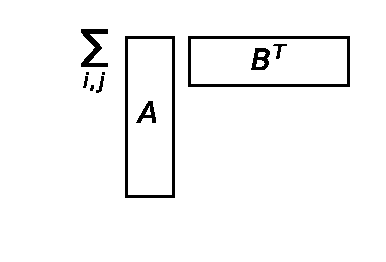
\includegraphics[width=130mm]{Results/normDifferenceFromUSVs.pdf}
\caption[Exact norm of difference]{Exact norm of difference via SVD}
\label{fig:normDifferenceFromUSVs}
\end{figure}

For very large datasets, the SVDs may be obtained using a random algorithm reviewed extensively in an article by Halko et al.~\cite{Halko2011}. The number of singular values will then be truncated to the $l$ largest values, similar to finding an $\epsilon$-rank approximation. In section~\ref{sec:Techniques Approximate SVD via Dimension Reduction}, we will also apply this technique to our generated fields. The resulting norm will no longer be exact, but the error can be made arbitrarily small by adjusting $l$ and $\epsilon$

\subsection{Protocol}
\label{sec:Introduction/Protocol}

Lorem ipsum dolor sit amet, consectetur adipiscing elit, sed do eiusmod tempor incididunt ut labore et dolore magna aliqua. Ut enim ad minim veniam, quis nostrud exercitation ullamco laboris nisi ut aliquip ex ea commodo consequat. Duis aute irure dolor in reprehenderit in voluptate velit esse cillum dolore eu fugiat nulla pariatur. Excepteur sint occaecat cupidatat non proident, sunt in culpa qui officia deserunt mollit anim id est laborum.

\begin{figure}[H]
\centering
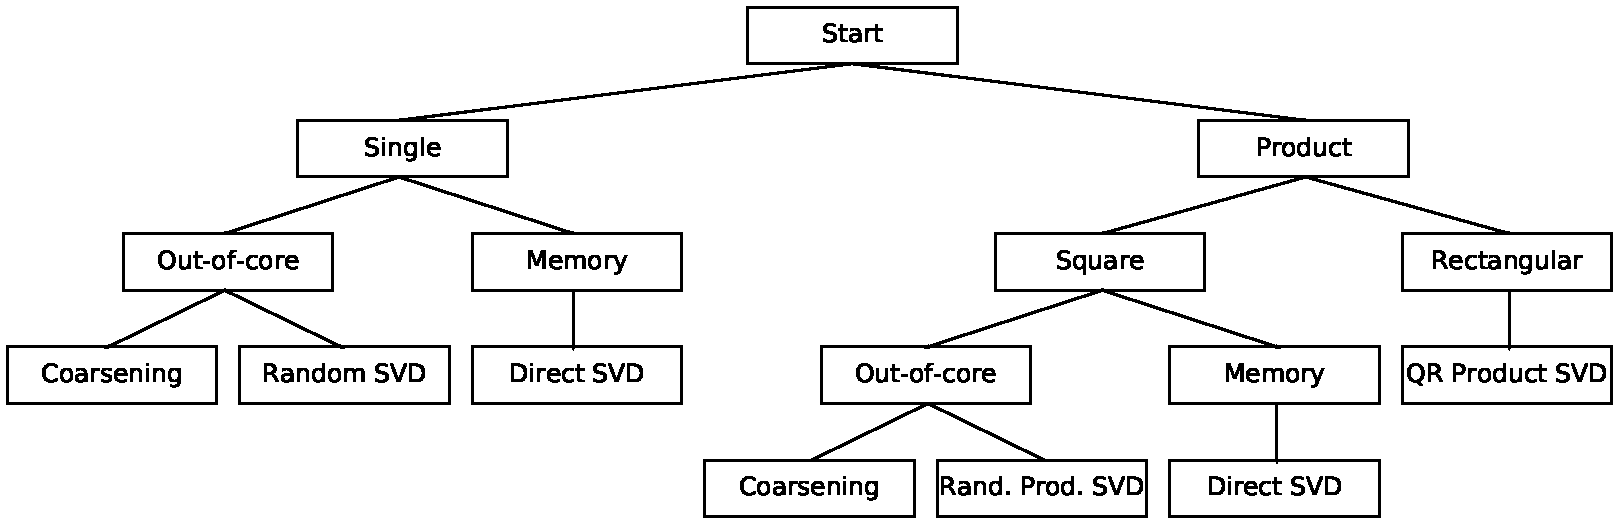
\includegraphics[width=120mm]{Results/FlowDiagram.pdf}
\caption{This is a figure.}
\label{fig:FlowDiagram}
\end{figure}

Lorem ipsum dolor sit amet, consectetur adipiscing elit, sed do eiusmod tempor incididunt ut labore et dolore magna aliqua. Ut enim ad minim veniam, quis nostrud exercitation ullamco laboris nisi ut aliquip ex ea commodo consequat. Duis aute irure dolor in reprehenderit in voluptate velit esse cillum dolore eu fugiat nulla pariatur. Excepteur sint occaecat cupidatat non proident, sunt in culpa qui officia deserunt mollit anim id est laborum.

%%%%%%%%%%%%%%%%%%%%%%%%%%%%%%%%%%%%%%%%%%
\section{Materials and Methods}
\label{sec:Materials and Methods}

%Materials and Methods should be described with sufficient details to allow others to replicate and build on published results. Please note that publication of your manuscript implicates that you must make all materials, data, computer code, and protocols associated with the publication available to readers. Please disclose at the submission stage any restrictions on the availability of materials or information. New methods and protocols should be described in detail while well-established methods can be briefly described and appropriately cited.

%Research manuscripts reporting large datasets that are deposited in a publicly available database should specify where the data have been deposited and provide the relevant accession numbers. If the accession numbers have not yet been obtained at the time of submission, please state that they will be provided during review. They must be provided prior to publication.

%Interventionary studies involving animals or humans, and other studies require ethical approval must list the authority that provided approval and the corresponding ethical approval code. 

Lorem ipsum dolor sit amet, consectetur adipiscing elit, sed do eiusmod tempor incididunt ut labore et dolore magna aliqua. Ut enim ad minim veniam, quis nostrud exercitation ullamco laboris nisi ut aliquip ex ea commodo consequat. Duis aute irure dolor in reprehenderit in voluptate velit esse cillum dolore eu fugiat nulla pariatur. Excepteur sint occaecat cupidatat non proident, sunt in culpa qui officia deserunt mollit anim id est laborum.

\subsection{Spatio-Temporal Fields}
\label{sec:Materials and Methods/Spatio-Temporal Fields}

In domains such a climate science and phenology, datasets are typically spatial fields, e.g. of temperature. In these fields, values vary slowly and neighbouring points are not entirely independent of one another, neither in space nor in time~\cite{Eshel2011}. Then, there is a high level of autocorrelation and the field has large scale structure. Such redundancy means the dataset is rank deficient.

To compare our techniques and to find a relation between performance and structure scale, we need to be able to generate fields which resemble those often encountered in real-world applications. In particular, we will concern ourselves with fields which combine some level of autocorrelation with some randomness. Real-valued \textit{Gaussian Random Fields} are particularly useful because their structure scale can be captured in a single parameter, as shown in figure~\ref{fig:GaussianRandomField}. For two dimensional spatial fields, rotational invariance is assumed. Then, the spectrum of such fields follows the power law described by $P(k) = c_{0} \, |\vec{k}|^{-\alpha}$ where $\vec{k}$ is the wavevector and $\alpha$ the parameter which controls the level of autocorrelation.

\begin{figure}[H]
\centering
\subfloat[$\alpha = 1$]{\label{fig:GaussianRandomFieldSize400Alpha1.pdf}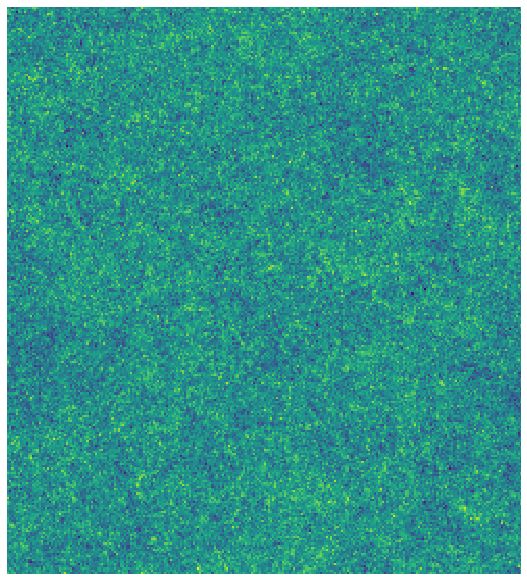
\includegraphics[scale=.4]{Results/GaussianRandomFieldSize400Alpha1.pdf}}
\hspace{8mm}
\subfloat[$\alpha = 3$]{\label{fig:GaussianRandomFieldSize400Alpha3.pdf}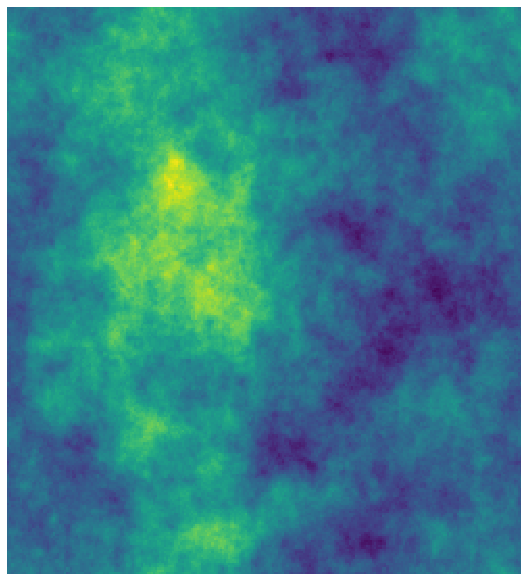
\includegraphics[scale=.4]{Results/GaussianRandomFieldSize400Alpha3.pdf}}
\hspace{8mm}
\subfloat[$\alpha = 5$]{\label{fig:GaussianRandomFieldSize400Alpha5.pdf}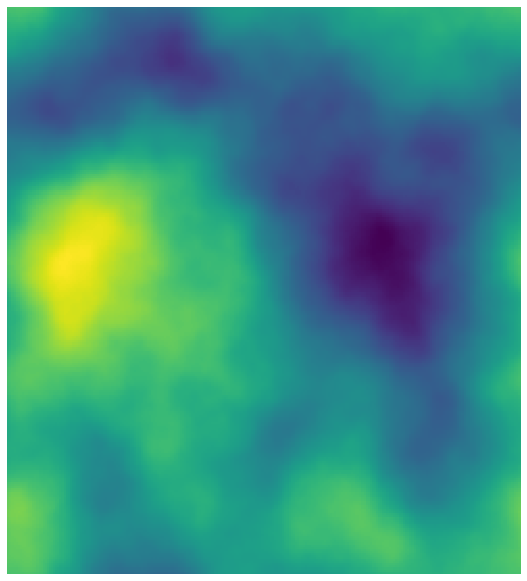
\includegraphics[scale=.4]{Results/GaussianRandomFieldSize400Alpha5.pdf}}
\caption{Gaussian Random Fields for various $\alpha$'s}
\label{fig:GaussianRandomField}
\end{figure}

In many real-world applications, the analysis of a field does not only involve a single time period but includes data over multiple weeks, months or years. Then, we are interested in finding patterns which occur frequently. The \textit{maximum covariance analysis} (MCA) and \textit{canonical correlation analysis} (CCA) examine the cross-covariance matrix of two datasets and find patterns which occur frequently and simultaneously~\cite{Eshel2011, Storch1999}. Such a pattern, or mode, is a combination of a left- and a right basis vector. One technique to find these modes is to perform an SVD on the product of the standardised datasets. In some domains, the term SVD is used synonymously with MCA. In an MCA, modes are found where the left- and the right vector covary maximally, whereas in a CCA, they correlate maximally~\cite{Bretherton1992}.

Just as there is spatial autocorrelation, there is temporal autocorrelation, when the values of the field over the entire time period do not change drastically. In principle, there can be different levels of autocorrelation over time and over space. However, for simplicity, in this article we will use the same $\alpha$ to determine the level of autocorrelation in all dimensions.

\subsection{Autocorrelation}
\label{sec:Materials and Methods/Autocorrelation}

In spatial data analysis, other measures of autocorrelation are used \cite{Eshel2011, Storch1999}. These include Moran's $I$ and the $\Gamma$ index~\cite{Moran1950, Hubert1981, PySAL}. Finally, one can devise a measure from the singular values. Each singular value indicates the amount of variance explained by its associated mode. For fields with autocorrelation, the sorted list of singular values decays quickly. One can try to fit a power law to this list and estimate the exponent, which we will call $\beta$. %While the power spectrum gives the data in terms of harmonics, an SVD gives it in terms of empirical observed functions. Therefore, the singular values will always decay more quickly than the amplitude of the wavevectors, and $\beta$ will always be larger than $\alpha$.
All these measures give an indication of the scale of the structure in the field and the level of autocorrelation in the data. Figure~\ref{fig:plotGammaAndMoransIAndBeta} plots them as a function of $\alpha$ for various generated Gaussian Random Fields.

\begin{figure}[H]
\centering
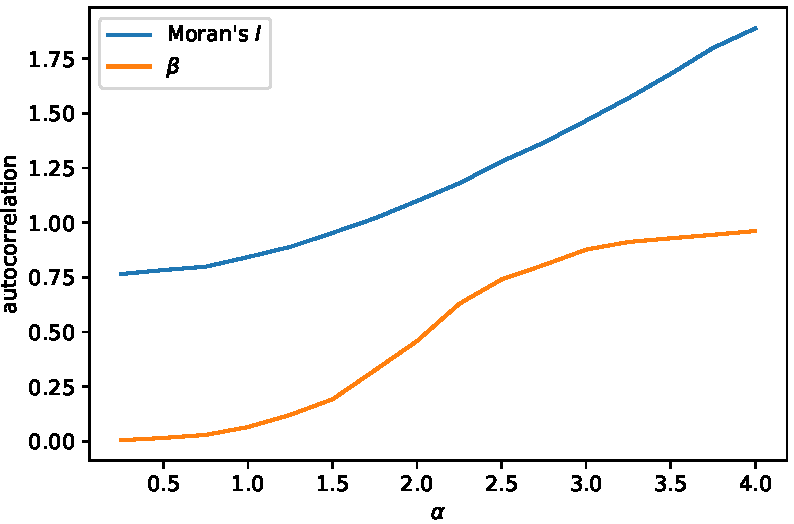
\includegraphics[width=80mm]{Results/plotMoransIAndBeta.pdf}
\caption[Various measures of autocorrelation]{Measures of autocorrelation as a function of $\alpha$}
\label{fig:plotGammaAndMoransIAndBeta}
\end{figure}

Lorem ipsum dolor sit amet, consectetur adipiscing elit, sed do eiusmod tempor incididunt ut labore et dolore magna aliqua. Ut enim ad minim veniam, quis nostrud exercitation ullamco laboris nisi ut aliquip ex ea commodo consequat. Duis aute irure dolor in reprehenderit in voluptate velit esse cillum dolore eu fugiat nulla pariatur. Excepteur sint occaecat cupidatat non proident, sunt in culpa qui officia deserunt mollit anim id est laborum.

%%%%%%%%%%%%%%%%%%%%%%%%%%%%%%%%%%%%%%%%%%
\section{Results}

%This section may be divided by subheadings. It should provide a concise and precise description of the experimental results, their interpretation as well as the experimental conclusions that can be drawn.
%\begin{quote}
%This section may be divided by subheadings. It should provide a concise and precise description of the experimental results, their interpretation as well as the experimental conclusions that can be drawn.
%\end{quote}

This section lists four SVD related implementations to analyse large datasets by exploiting autocorrelation and rank deficiency.

\subsection{Exact Product SVD via QR Decomposition}
\label{sec:Materials and Methods/Exact Product SVD via QR Decomposition}

In real-world applications, one often wants to find the relation between two fields. Analyses such as the MCA and CCA discussed in section~\ref{sec:Introduction Spatio-Temporal Fields} rely on performing an SVD of the cross-covariance matrix of the two fields. Take two input datasets with the various spatial gridpoints as rows and the sample of recorded values over time as columns. Centering and multiplying these gives the cross-covariance matrix. For highly rectangular matrices, when there are many spatial gridpoint but few temporal samples, the resulting cross-covariance matrix is inefficiently large and obviously rank deficient. Performing a rank decomposition, such as the \textit{QR decomposition}, allows one to do the SVD in an efficient manner~\cite{Chan1982, Tygert2017}. As shown in figure~\ref{fig:qrProductSVD}, the result is mathematically identical to the full SVD, which means that the difference will be at machine-precision.

\begin{figure}[H]
\centering
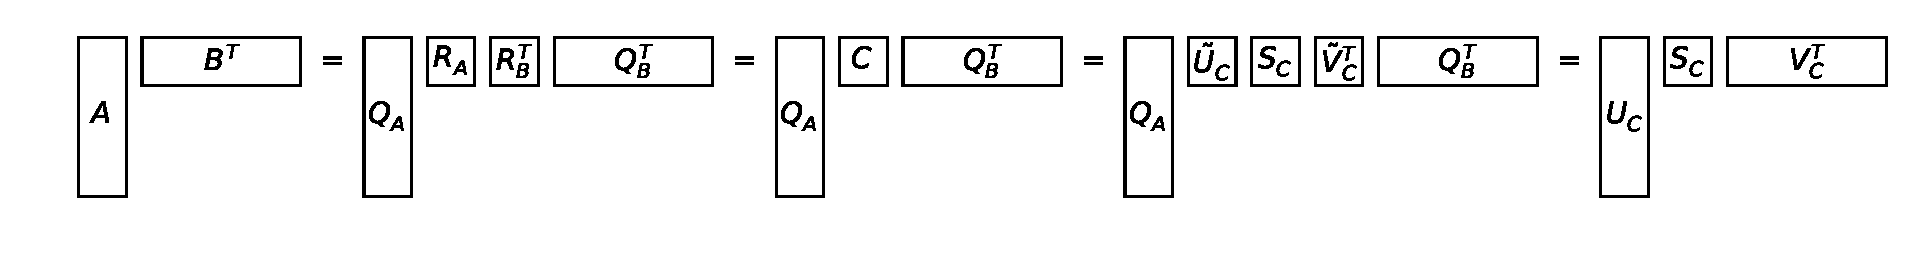
\includegraphics[width=120mm]{Results/qrProductSVD.pdf}
\caption[Exact SVD via QR decomposition]{Exact SVD of a product via QR decomposition}
\label{fig:qrProductSVD}
\end{figure}

\subsection{Case Study using SI-x and AVHRR Data}
\label{sec:Materials and Methods/Case Study using SI-x and AVHRR Data}

Phenology is the science that studies the timings of recurring biological events such as leafing and blooming as well as their causes and variations in space and time. Time series of remotely sensed images can be used to derive various land surface phenological metrics. One of these metrics is the so-called Start of Season (SOS), which indicates the beginning of photosynthetic activity in plants. In this section, we use a SOS product made for the US by processing time series of the Advanced Very High Resolution Radiometer sensor~\cite{Reed1994}. The Extended Spring Indices (SI-x) are a suite of models that transform daily temperatures into consistent phenological metrics~\cite{Schwartz2013}. We use a new long-term ($1989$ to $2014$) and high spatial resolution ($1$km) version of the Bloom index, which was recently generated for the US by adapting the SI-x models to a cloud computing environment~\cite{Izquierdo2015}. Estimated over a square subsection of the USA, we find the Bloom field to have $\alpha \approx 1.4$ and the SOS field to have $\alpha \approx 0.6$~\cite{Bogaardt2018}.

\subsection{Approximate SVD via Spatial Coarsening}
\label{sec:Materials and Methods/Approximate SVD via Spatial Coarsening}

Although the QR decomposition works well for two rectangular matrices, sometimes the input data is large and square. Performing an SVD on such large datasets will be time consuming. When a spatial field has large scale structure, the values of neighbouring cells do not change drastically. Perhaps these cells can be aggregated together to produce a smaller dataset which still faithfully describes the original field. In this section, we coarsen various Gaussian Random Fields by averaging patches of neighbouring gridpoints. We then compare the result with the full calculation.

\begin{figure}[H]
\centering
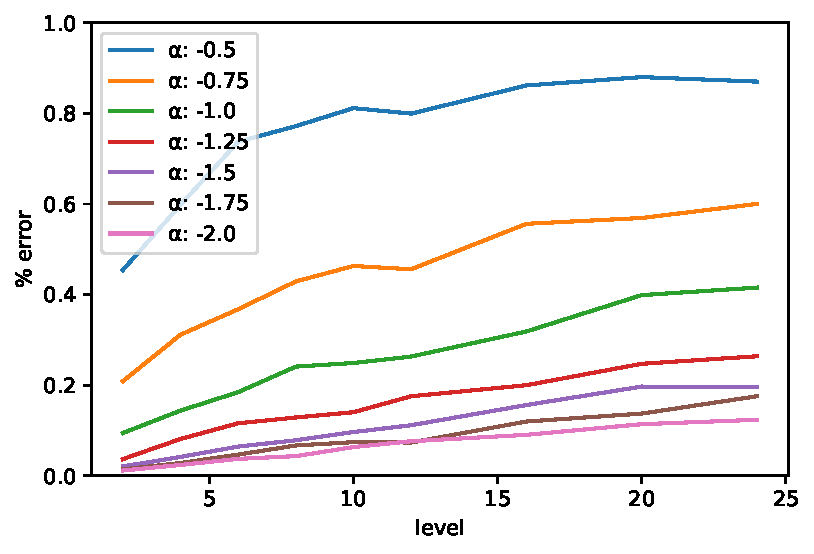
\includegraphics[width=100mm]{Results/plotSingleSpatialFieldViaCoarsening.pdf}
\caption[Error after coarsening a spatial field]{Error after coarsening a spatial field for various $\alpha$'s}
\label{fig:plotSingleSpatialFieldViaCoarsening}
\end{figure}

Figure~\ref{fig:plotSingleSpatialFieldViaCoarsening} shows the percentage error in a coarsening process for matrices of various $\alpha$'s and different windows sizes. The error is determined as the norm of the difference between the original matrix and the coarsened version, divided by the norm of the original~\cite{Bogaardt2018}. Note that a field with high autocorrelation ($\alpha=2$) differs only by a few percent from one $25$ times smaller (level $= 5$).

\subsection{Approximate SVD via Dimension Reduction}
\label{sec:Materials and Methods/Approximate SVD via Dimension Reduction}

The spatial coarsening process is intuitive and easy to implement. It is not, however, the most efficient way to reduce the size of a dataset. Dimension reduction refers to discarding modes which contribute little to the variance in a dataset. As mentioned in section~\ref{sec:Introduction Matrix Size and Rank Decomposition}, an SVD is precisely the procedure used to find modes which explain as much variance as possible. Discarding the smallest singular values, therefore, gives the best lower rank approximation~\cite{Eckart1936, Martinsson2016}. Performing an SVD on a large dataset, however, is computationally costly. The \textit{randomised dimension reduction} process, reviewed extensively in the article by Halko et al., is more efficient~\cite{Halko2011, Li2016}.

As depicted in figure~\ref{fig:reduceSizeRandomisedSquare}, this process reduces the input matrix to a smaller square matrix of $l$ by $l$. It also gives two projection matrices which can bring the rows and columns of this smaller matrix back to the bases of the original input. It is a randomised procedure to get an $\epsilon$-rank approximation and, therefore, the error will be at the order of the size of the largest truncated singular value~\cite{Martinsson2016, Halko2011}. Our \textit{Jupyter Notebook} provides more details~\cite{Bogaardt2018}.

\begin{figure}[H]
\centering
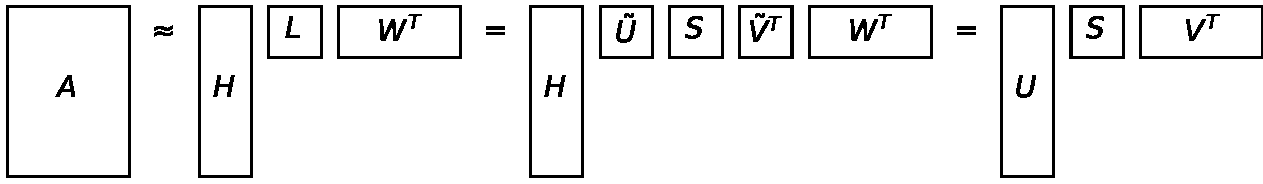
\includegraphics[width=120mm]{Results/reduceSizeRandomisedSquare.pdf}
\caption[Approximate randomised SVD]{Approximate SVD via dimension reduction}
\label{fig:reduceSizeRandomisedSquare}
\end{figure}

In the review article by Halko et al. on randomised dimension reduction, it is suggested to oversample the reduction. This is because the error introduced in the process is of the same order as the size of the last sampled singular value. If one is interested in the k dominant modes, reducing to a k + l, for some small l, rank approximation will ensure the first k modes are approximated quite well. Indeed, as seen below, the more modes one is interested in, the larger the difference compared with the original matrix.% quote:"the failure probability decreases superexponentially with the oversampling parameter p".

\subsection{Case Study using ERA-5 Data}
\label{sec:Materials and Methods/Case Study using ERA-5 Data}

Lorem ipsum dolor sit amet, consectetur adipiscing elit, sed do eiusmod tempor incididunt ut labore et dolore magna aliqua. Ut enim ad minim veniam, quis nostrud exercitation ullamco laboris nisi ut aliquip ex ea commodo consequat. Duis aute irure dolor in reprehenderit in voluptate velit esse cillum dolore eu fugiat nulla pariatur. Excepteur sint occaecat cupidatat non proident, sunt in culpa qui officia deserunt mollit anim id est laborum.

\subsection{Approximate Product SVD via Spatial Coarsening}
\label{sec:Materials and Methods/Approximate SVD via Spatial Coarsening}

We can also coarsen two different fields before analysing their cross-covariance matrix. Figure~\ref{fig:plotProductSpatialTemporalFieldsViaCoarsening} shows the percentage error for various generated matrices. Due to the multiplication step in this analysis, the typical error as a result of coarsening is larger than before. As expected, the level of autocorrelation plays an important part, with larger $\alpha$'s leading to less error. The amount of error during the coarsening process will likely also depend on the similarity between the two datasets. We leave this aspect for further research.

\begin{figure}[H]
\centering
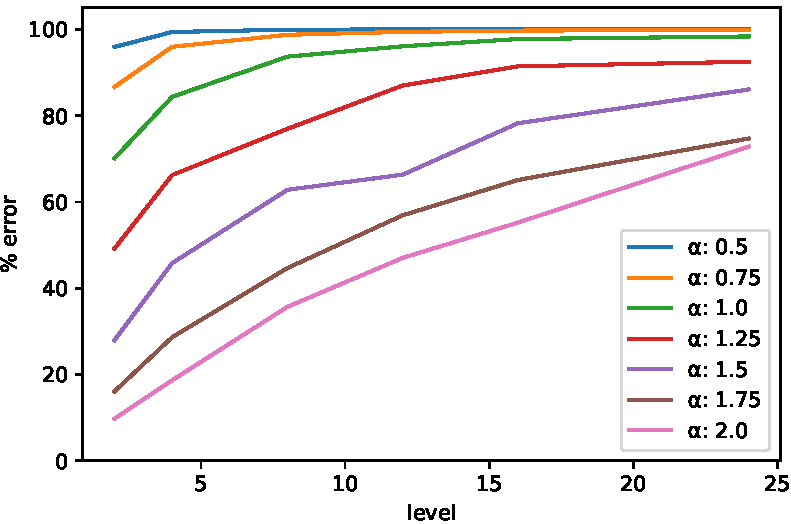
\includegraphics[width=100mm]{Results/plotProductSpatialTemporalFieldsViaCoarsening.pdf}
\caption[Error after coarsening product of fields]{Error after coarsening the product of two fields}
\label{fig:plotProductSpatialTemporalFieldsViaCoarsening}
\end{figure}

The coarsening process can speed up the calculation of the SVD, and there are additional benefits. When a target level of accuracy is set and there is an a priori estimate of the level of autocorrelation of the fields, the data collection process can be optimised. Knowing in advance at what resolution to gather data can help save time. Furthermore, in domains were satellite data is used, datasets are often not very detailed because the imaging resolution is low. Unlike local analyses of developed countries, where high resolution data is becoming more accessible, for continental or global analyses, coarse spatial resolution data may simply be the only option.

\subsection{Approximate Product SVD via Dimension Reduction}
\label{sec:Materials and Methods/Approximate SVD via Dimension Reduction}

The randomised dimension reduction process can also be applied to the MCA or CCA analysis of two spatio-temporal fields. Similar to the QR product SVD, it has the advantage that the SVD is applied to a small $l$ by $l$ matrix, as seen in figure~\ref{fig:randomisedSquareProductSVD}.

\begin{figure}[H]
\centering
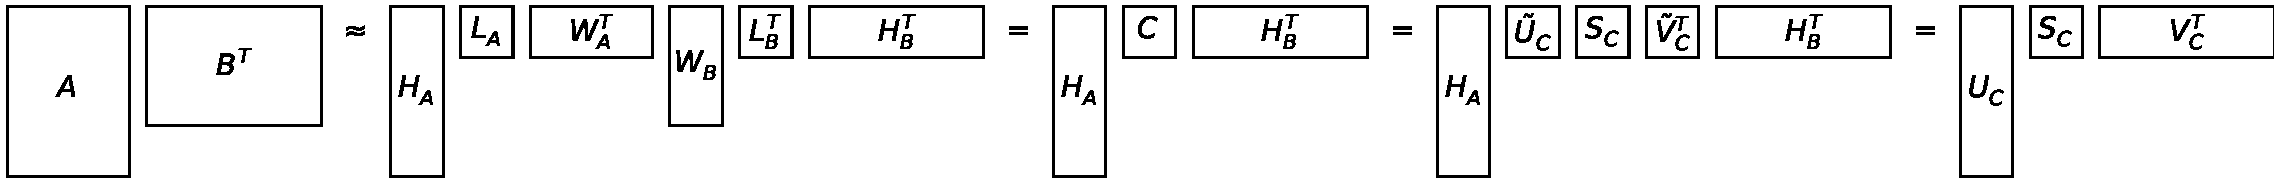
\includegraphics[width=120mm]{Results/randomisedSquareProductSVD.pdf}
\caption[Approximate product SVD]{Approximate SVD for product of two fields}
\label{fig:randomisedSquareProductSVD}
\end{figure}

To see the effect of dimension reduction on such a matrix product, let's generate various Gaussian Random Fields and compare their cross-correlation matrix with a reduced version. Figure~\ref{fig:plotRandomisedSizeReducedMatrixProduct} shows that the results are terrible for fields with a small $\alpha$, but high levels of autocorrelation allow for substantial savings in computation time without acquiring much error.

\begin{figure}[H]
\centering
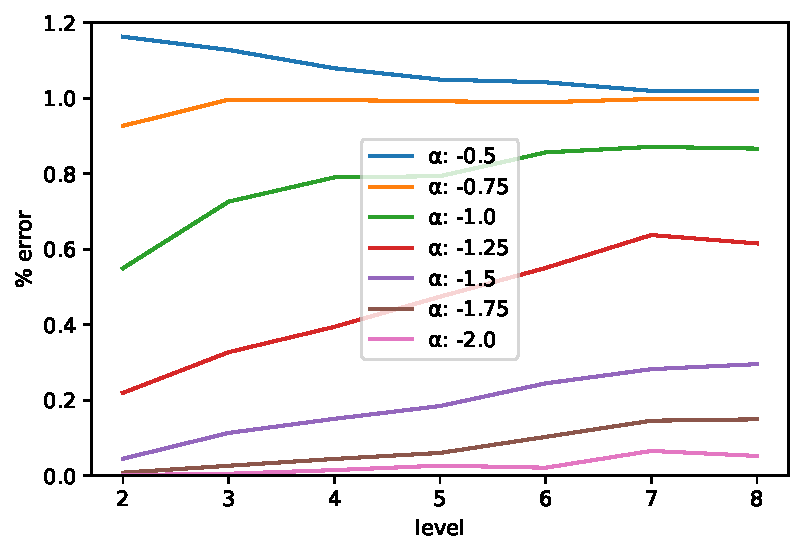
\includegraphics[width=100mm]{Results/plotRandomisedSizeReducedMatrixProduct.pdf}
\caption[Error after SVD]{Error after SVD of approximated fields}
\label{fig:plotRandomisedSizeReducedMatrixProduct}
\end{figure}

Again, we performed our analysis with two generated fields which correlated highly. Whether this correlation influences the amount of error after dimension reduction is left open.

The reduction of the number of dimensions of each input dataset is actually advised by some researchers, as a method to filter out noise~\cite{Barnett1987}. Especially when the number of temporal samples is small, outliers and random fluctuations could affect the result~\cite{Bretherton1992}. This is because any statistical analysis will choose its regression-coefficients so as to optimize the fit. It may occur that two noise-vectors in the two fields coincidentally covary and show up as dominant modes. Prefiltering can alleviate this risk.

When a dataset is too large to fit in memory, the time of transferring the matrix from storage often takes longer than the actual analysis~\cite{Halko2011}. The additional benefit of this procedure is that the randomized technique requires only a constant number of passes over the data, reducing storage communication time.

\subsection{Case Study using JRA-55 Data}
\label{sec:Materials and Methods/Case Study using JRA-55 Data}

Lorem ipsum dolor sit amet, consectetur adipiscing elit, sed do eiusmod tempor incididunt ut labore et dolore magna aliqua. Ut enim ad minim veniam, quis nostrud exercitation ullamco laboris nisi ut aliquip ex ea commodo consequat. Duis aute irure dolor in reprehenderit in voluptate velit esse cillum dolore eu fugiat nulla pariatur. Excepteur sint occaecat cupidatat non proident, sunt in culpa qui officia deserunt mollit anim id est laborum.

%%%%%%%%%%%%%%%%%%%%%%%%%%%%%%%%%%%%%%%%%%
%\subsection{Subsection}

%\subsubsection{Subsubsection}

%Bulleted lists look like this:
%\begin{itemize}[leftmargin=*,labelsep=5.8mm]
%\item	First bullet
%\item	Second bullet
%\item	Third bullet
%\end{itemize}

%Numbered lists can be added as follows:
%\begin{enumerate}[leftmargin=*,labelsep=4.9mm]
%\item	First item 
%\item	Second item
%\item	Third item
%\end{enumerate}

%The text continues here.

%\subsection{Figures, Tables and Schemes}

%All figures and tables should be cited in the main text as Figure 1, Table 1, etc.

%\begin{figure}[H]
%\centering
%
\includegraphics[width=2 cm]{Definitions/logo-mdpi}
%\caption{This is a figure, Schemes follow the same formatting. If there are multiple panels, they should be listed as: (\textbf{a}) Description of what is contained in the first panel. (\textbf{b}) Description of what is contained in the second panel. Figures should be placed in the main text near to the first time they are cited. A caption on a single line should be centered.}
%\end{figure}   

%\begin{table}[H]
%\caption{This is a table caption. Tables should be placed in the main text near to the first time they are cited.}
%\centering
%% \tablesize{} %% You can specify the fontsize here, e.g.  \tablesize{\footnotesize}. If commented out \small will be used.
%\begin{tabular}{ccc}
%\toprule
%\textbf{Title 1}	& \textbf{Title 2}	& \textbf{Title 3}\\
%\midrule
%entry 1		& data			& data\\
%entry 2		& data			& data\\
%\bottomrule
%\end{tabular}
%\end{table}

%\subsection{Formatting of Mathematical Components}

%This is an example of an equation:

%\begin{equation}
%a + b = c
%\end{equation}
%% If the documentclass option "submit" is chosen, please insert a blank line before and after any math environment (equation and eqnarray environments). This ensures correct linenumbering. The blank line should be removed when the documentclass option is changed to "accept" because the text following an equation should not be a new paragraph. 

%Please punctuate equations as regular text. Theorem-type environments (including propositions, lemmas, corollaries etc.) can be formatted as follows:
%% Example of a theorem:
%\begin{Theorem}
%Example text of a theorem.
%\end{Theorem}

%The text continues here. Proofs must be formatted as follows:

%% Example of a proof:
%\begin{proof}[Proof of Theorem 1]
%Text of the proof. Note that the phrase `of Theorem 1' is optional if it is clear which theorem is being referred to.
%\end{proof}
%The text continues here.

%%%%%%%%%%%%%%%%%%%%%%%%%%%%%%%%%%%%%%%%%%
\section{Discussion}

%Authors should discuss the results and how they can be interpreted in perspective of previous studies and of the working hypotheses. The findings and their implications should be discussed in the broadest context possible. Future research directions may also be highlighted.

\subsection{Further Work}
\label{sec:Discussion/Further Work}

Much of the analysis here relies on a priori knowledge of the level of autocorrelation. If datasets are large, it would be nice to have an algorithm to estimate Moran's $I$, or another measure of autocorrelation, using only a small sample of the data. It may also be interesting to extend this research to fields other than the Gaussian Random Field. This type was chosen because its structure scale can be captured in a single parameter $\alpha$. Additionally, it would be an improvement to relax the assumption that the autocorrelation in the time direction is similar to that in the spatial directions. In fact, it may even be more realistic to have different levels of autocorrelation in the North-South and in the East-West direction.

Finally, note that, unlike the coarsening procedure, the dimension reduction is not applied on each spatial field for each time period, but rather on the entire spatially flattened timeseries. Therefore, the level of spatial autocorrelation may not be as important as the level of temporal autocorrelation. Further work can examine if better results are obtained when the dimension reduction is applied to the spatial part of the spatio-temporal fields, before it is flattened.

\subsection{Conclusion}
\label{sec:Discussion/Conclusion}

In conclusion, performing analyses at a coarse level can be beneficial when data collection is difficult%\footnote{In the \textit{Jupyter Notebook} accompanying this article, we applied the techniques to real datasets of phenological metrics and obtained similar results to those predicted by the Gaussian Random Fields~\cite{Bogaardt2018}.}
. Using the randomised dimension reduction can be helpful for datasets which are too large for internal memory. And, finally, rank decomposition may speed up calculations by splitting datasets into square, full rank matrices together with left- and right orthonormal rotation matrices. Once the analysis is performed on the smaller matrix, the output can be rotated back to the original bases, often saving computation time.

%%%%%%%%%%%%%%%%%%%%%%%%%%%%%%%%%%%%%%%%%%
%\section{Conclusions}

%This section is not mandatory, but can be added to the manuscript if the discussion is unusually long or complex.

%%%%%%%%%%%%%%%%%%%%%%%%%%%%%%%%%%%%%%%%%%
%\section{Patents}
%This section is not mandatory, but may be added if there are patents resulting from the work reported in this manuscript.

%%%%%%%%%%%%%%%%%%%%%%%%%%%%%%%%%%%%%%%%%%
\vspace{6pt} 

%%%%%%%%%%%%%%%%%%%%%%%%%%%%%%%%%%%%%%%%%%
%% optional
%\supplementary{The following are available online at \linksupplementary{s1}, Figure S1: title, Table S1: title, Video S1: title.}

% Only for the journal Methods and Protocols:
% If you wish to submit a video article, please do so with any other supplementary material.
% \supplementary{The following are available at \linksupplementary, Figure S1: title, Table S1: title, Video S1: title. A supporting video article is available at doi: link.}

%%%%%%%%%%%%%%%%%%%%%%%%%%%%%%%%%%%%%%%%%%
\authorcontributions{Conceptualization, R.Z.; Methodology, L.B.; Software, L.B.; Validation, R.G., R.Z. and E.I.; Formal Analysis, L.B.; Investigation, L.B.; Resources, R.G., R.Z. and E.I.; Data Curation, R.G., R.Z. and E.I.; Writing—Original Draft Preparation, L.B.; Writing—Review \& Editing, R.G., R.Z. and E.I.; Visualization, L.B.; Supervision, R.G. and R.Z.; Project Administration, R.G.; Funding Acquisition, R.Z.}

%%%%%%%%%%%%%%%%%%%%%%%%%%%%%%%%%%%%%%%%%%
\funding{Please add: ``This research received no external funding'' or ``This research was funded by [name of funder] grant number [xxx].'' Check carefully that the details given are accurate and use the standard spelling of funding agency names at \url{https://search.crossref.org/funding}, any errors may affect your future funding.}

%%%%%%%%%%%%%%%%%%%%%%%%%%%%%%%%%%%%%%%%%%
%\acknowledgments{In this section you can acknowledge any support given which is not covered by the author contribution or funding sections. This may include administrative and technical support, or donations in kind (e.g. materials used for experiments).}

%%%%%%%%%%%%%%%%%%%%%%%%%%%%%%%%%%%%%%%%%%
\conflictsofinterest{The authors declare no conflict of interest. The founding sponsors had no role in the design of the study; in the collection, analyses, or interpretation of data; in the writing of the manuscript, and in the decision to publish the results.} 

%%%%%%%%%%%%%%%%%%%%%%%%%%%%%%%%%%%%%%%%%%
%% optional
\abbreviations{The following abbreviations are used in this manuscript:\\

\noindent 
\begin{tabular}{@{}ll}
SVD & Singular value decomposition\\
SI-x & Extended spring indices\\
AVHRR & Advanced very-high-resolution radiometer\\
ERA-5 & European reanalysis\\
JRA-55 & Japanese 55-year reanalysis
\end{tabular}}

%%%%%%%%%%%%%%%%%%%%%%%%%%%%%%%%%%%%%%%%%%
%% optional
%\appendixtitles{no} %Leave argument "no" if all appendix headings stay EMPTY (then no dot is printed after "Appendix A"). If the appendix sections contain a heading then change the argument to "yes".
%\appendixsections{multiple} %Leave argument "multiple" if there are multiple sections. Then a counter is printed ("Appendix A"). If there is only one appendix section then change the argument to "one" and no counter is printed ("Appendix").
%\appendix
%\section{}
%\subsection{}
%The appendix is an optional section that can contain details and data supplemental to the main text. For example, explanations of experimental details that would disrupt the flow of the main text, but nonetheless remain crucial to understanding and reproducing the research shown; figures of replicates for experiments of which representative data is shown in the main text can be added here if brief, or as Supplementary data. Mathematical proofs of results not central to the paper can be added as an appendix.

%\section{}
%All appendix sections must be cited in the main text. In the appendixes, Figures, Tables, etc. should be labeled starting with `A', e.g., Figure A1, Figure A2, etc. 

%%%%%%%%%%%%%%%%%%%%%%%%%%%%%%%%%%%%%%%%%%
% Citations and References in Supplementary files are permitted provided that they also appear in the reference list here. 

%=====================================
% References, variant A: internal bibliography
%=====================================
%\reftitle{References}
%\begin{thebibliography}{999}
% Reference 1
%\bibitem[Author1(year)]{ref-journal}
%Author1, T. The title of the cited article. {\em Journal Abbreviation} {\bf 2008}, {\em 10}, 142-149, DOI.
% Reference 2
%\bibitem[Author2(year)]{ref-book}
%Author2, L. The title of the cited contribution. In {\em The Book Title}; Editor1, F., Editor2, A., Eds.; Publishing House: City, Country, 2007; pp. 32-58, ISBN.
%\end{thebibliography}

% The following MDPI journals use author-date citation: Arts, Econometrics, Economies, Genealogy, Humanities, IJFS, JRFM, Laws, Religions, Risks, Social Sciences. For those journals, please follow the formatting guidelines on http://www.mdpi.com/authors/references
% To cite two works by the same author: \citeauthor{ref-journal-1a} (\citeyear{ref-journal-1a}, \citeyear{ref-journal-1b}). This produces: Whittaker (1967, 1975)
% To cite two works by the same author with specific pages: \citeauthor{ref-journal-3a} (\citeyear{ref-journal-3a}, p. 328; \citeyear{ref-journal-3b}, p.475). This produces: Wong (1999, p. 328; 2000, p. 475)

%=====================================
% References, variant B: external bibliography
%=====================================
\externalbibliography{yes}
\bibliography{Bibliography}

%%%%%%%%%%%%%%%%%%%%%%%%%%%%%%%%%%%%%%%%%%
%% optional
%\sampleavailability{Samples of the compounds ...... are available from the authors.}

%% for journal Sci
%\reviewreports{\\
%Reviewer 1 comments and authors’ response\\
%Reviewer 2 comments and authors’ response\\
%Reviewer 3 comments and authors’ response
%}

%%%%%%%%%%%%%%%%%%%%%%%%%%%%%%%%%%%%%%%%%%
\end{document}

